\documentclass[tikz,border=2pt]{standalone}
\usepackage{amsmath}
\usepackage{pgfplots}
\pgfplotsset{compat=1.18}
\usetikzlibrary{arrows.meta}
\begin{document}
% Building a ggplot in three steps with the series 2017-2021: Transport 33 34 33 29 30 (black points),
% Buildings 24 23 22 21 20 (red points); p1 = one layer, p2 = p1 + second layer, p3 = p2 + ylab() + ggtitle().
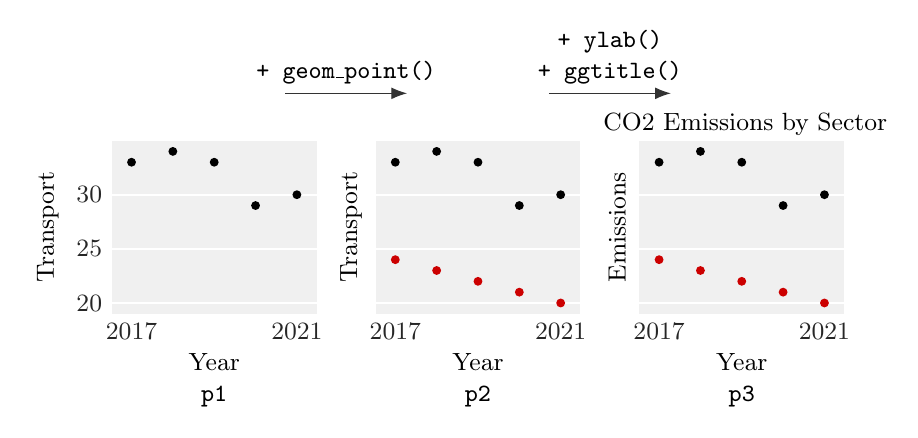
\begin{tikzpicture}[font=\small, >={Latex[length=2mm]},
  code/.style={font=\small\ttfamily, inner sep=1pt}]
  \def\pw{2.6}  % panel width
  \def\ph{2.2}  % panel height
  % map year 2017..2021 to 0.25..\pw-0.25 and emissions 19..35 to 0..\ph
  \newcommand{\px}[1]{(0.25+(#1-2017)*(\pw-0.5)/4)}
  \newcommand{\py}[1]{((#1-19)*\ph/16)}
  \newcommand{\panel}[4]{% #1 x-shift, #2 y label, #3 show red (1/0), #4 title
    \begin{scope}[shift={(#1,0)}]
      \fill[gray!12] (0,0) rectangle (\pw,\ph);
      \foreach \v in {20,25,30} {
        \draw[white, thick] (0,{\py{\v}}) -- (\pw,{\py{\v}});
        \ifdim#1pt=0pt \node[anchor=east, gray!30!black] at (0,{\py{\v}}) {\v};\fi
      }
      \foreach \t/\v in {2017/33,2018/34,2019/33,2020/29,2021/30}
        \fill[black] ({\px{\t}},{\py{\v}}) circle (1.6pt);
      \ifnum#3=1
        \foreach \t/\v in {2017/24,2018/23,2019/22,2020/21,2021/20}
          \fill[red!80!black] ({\px{\t}},{\py{\v}}) circle (1.6pt);
      \fi
      \node[anchor=north, gray!30!black] at ({\px{2017}},0) {2017};
      \node[anchor=north, gray!30!black] at ({\px{2021}},0) {2021};
      \node[anchor=north] at (0.5*\pw,-0.38) {Year};
      \node[rotate=90, anchor=south] at ({\ifdim#1pt=0pt -0.55\else -0.05\fi},0.5*\ph) {#2};
      \node[anchor=south west, inner sep=1pt] at (-0.5,\ph+0.02) {#4};
    \end{scope}}
  \panel{0}{Transport}{0}{}
  \panel{3.35}{Transport}{1}{}
  \panel{6.7}{Emissions}{1}{CO2 Emissions by Sector}
  % names below the panels
  \node[code] at (0.5*\pw,-1.05) {p1};
  \node[code] at (3.35+0.5*\pw,-1.05) {p2};
  \node[code] at (6.7+0.5*\pw,-1.05) {p3};
  % step arrows above the panels
  \draw[->, gray!40!black] (\pw-0.4,\ph+0.6) -- (3.35+0.4,\ph+0.6);
  \node[code, anchor=south] at ({(\pw+3.35)/2},\ph+0.68) {+ geom\_point()};
  \draw[->, gray!40!black] (3.35+\pw-0.4,\ph+0.6) -- (6.7+0.4,\ph+0.6);
  \node[code, anchor=south, align=center] at ({(3.35+\pw+6.7)/2},\ph+0.68) {+ ylab()\\+ ggtitle()};
\end{tikzpicture}
\end{document}
